\subsection{FeSe diatomic molecule}
\label{subsection:fese}
Transition metal systems are often difficult to model due to the many orbital and possibly magnetic descriptors introduced by $d$ electrons. 
This is seen in the proliferation of models for transition metals, which include terms like spin-spin coupling, spin-orbital coupling, hopping, Hund's like coupling, and so on. 
Models containing all possible descriptors are unwieldy, and it is difficult to determine which degrees of freedom are needed for a minimal model to reproduce an interesting effect. 
Transition metal systems are challenging to describe using most electronic structure methods because of the strong electron correlations and multiple oxidation states possible in these systems. 
Fixed-node DMC has been shown to be a highly accurate method on transition metal materials in improving the description of the ground state properties and energy gaps~\cite{Foyevtsova2014, Wagner_Abbamonte, Zheng2015, Wagner2016}. In this section, we apply DMD using fixed-node DMC to quantify the importance of various interactions in a FeSe diatomic molecule with a bond length equal to that of the iron based superconductor, FeSe~\cite{kumar_crystal_2010}, in order to help identifying the descriptors that may be relevant in the bulk material.
\begin{figure*}[htb]
  \centering
  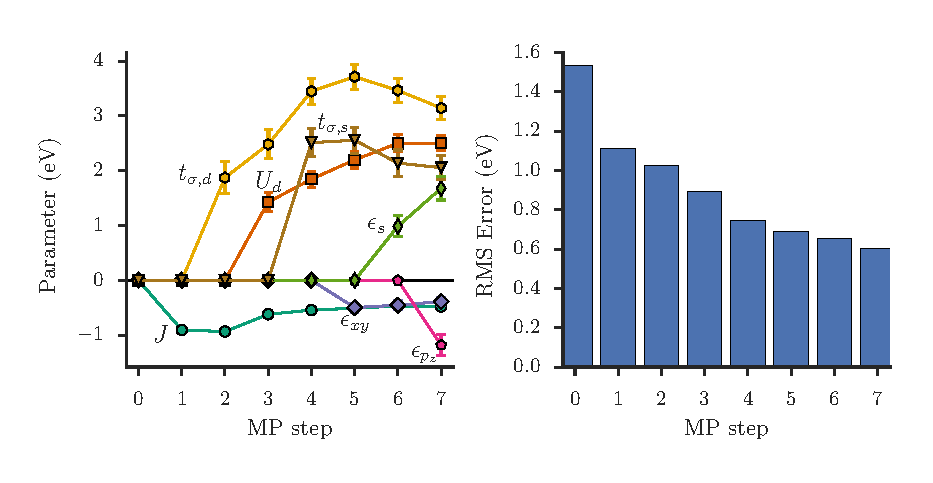
\includegraphics[width=0.8\textwidth]{./Figures/fese.eps}
  \caption{
    \label{fig:fese} 
    (Left) Parameter values for each fit generated in the MP algorithm, labeled at the step where they are included in the model. 
    A zero value indicates that parameter is not yet added to the model.
    The sign of $J$ is consistent with Hund's rules, and the signs of $t_{\sigma,d}$ and $t_{\sigma,s}$ are consistent with Se being located in positive $z$ with respect to Fe. 
    (Right) RMS error of each model generated by MP as the algorithm includes parameters. 
    The RMS error of the largest model considered was 0.61~eV.
  }
\end{figure*}

We considered a low-energy space spanned by the Se $4p$, Fe $3d$, and Fe $4s$ orbitals. We sampled singles and doubles excitations from a reference Slater determinant 
of Kohn-Sham orbitals taken from DFT calculations with PBE0 functional with total spin 0, 2, and 4, which were then multiplied by a Jastrow factor and further optimized using fixed-node DMC. 
After this procedure, 241 states were within a low energy window of 8 eV. 
Of these, eight states had a significant iron $4p$ component, which excludes them from the low-energy subspace. 
This leaves us with 233 states in the low-energy subspace.

We consider a set of 21 possible descriptors consisting of local operators on the iron $4s$, iron $3d$ states, and selenium $4p$ states, which is a total of 9 single-particle orbitals.
We use the same IAO construction as Section~\ref{subsection:1dhydrogen} to generate the basis for these operators.
At the one-body level, we consider orbital energy descriptors: 
\begin{align}
  &\epsilon_{s} n_s,&
  &\epsilon_{\pi,\mathrm{Se}} (n_{p_x} + n_{p_y}), &
  &\epsilon_{z} n_{p_z},&
  \nonumber \\
  &\epsilon_{z^2} n_{d_{z^2}},& 
  &\epsilon_{\pi,\mathrm{Fe}} (n_{d_{xz}} + n_{d_{yz}}).& 
  &\epsilon_{\delta} (n_{d_{xy}} + n_{d_{x^2-y^2}}),&
\end{align}
and the symmetry-allowed hopping terms:
\begin{align}
  &t_{\sigma,d} \sum_{\eta} \left( c_{d_{z^2},\eta}^{\dagger} c_{p_z,\eta} + \text{h.c.} \right),&
  &t_{\sigma,s} \sum_{\eta} \left(c_{s,\eta}^{\dagger}  c_{p_z,\eta} + \text{h.c.} \right),&
  &t_{\pi} \sum_{\eta} \left(c_{d_{xz},\eta}^{\dagger}  c_{p_x,\eta} + c_{d_{yz},\eta}^{\dagger}  c_{p_y,\eta} + \text{h.c.} \right).&
\end{align}
As before, $\eta$ represents the spin index. At the two-body level, we consider Hubbard interactions:
\begin{align}
  &U_p \sum_{i \in p} n_{i,\uparrow} n_{i,\downarrow},&
  &U_{d,\delta} \sum_{i\in \{d_{xy},d_{x^2-y^2}\}} n_{i,\uparrow} n_{i,\downarrow},&
  \nonumber \\
  &U_d \sum_{i \in d} n_{i,\uparrow} n_{i,\downarrow},&
  &U_{d,\pi} \sum_{i\in \{d_{xz},d_{yz}\}} n_{i,\uparrow} n_{i,\downarrow},&
  &U_{d_{z^2}} n_{d_{z^2},\uparrow} n_{d_{z^2},\downarrow},&
\end{align}
where $p$ refers to the Se-$4p$ orbitals and $d$ refers to the Fe-$3d$ orbitals. 
Importantly, we also account for the Hund's coupling terms for the iron atom:
\begin{align}
  &J \sum_{\substack{i\ne j \\i,j \in d}} S_i \cdot S_j,&
  &J_{\delta} S_{d_{xy}} \cdot S_{d_{x^2-y^2}},&
  &J_{\delta,d_{z^2}} (S_{d_{xy}} + S_{d_{x^2-y^2}}) \cdot S_{d_{z^2}},& \label{eqn:hund1}
  \nonumber \\
  &J_{\pi} S_{d_{xz}} \cdot S_{d_{yz}},&
  &J_{\pi,d_{z^2}} (S_{d_{xz}} + S_{d_{yz}}) \cdot S_{d_{z^2}}.&
  &J_{\pi,\delta} (S_{d_{xz}} + S_{d_{yz}}) \cdot (S_{d_{xy}} + S_{d_{x^2-y^2}}),&
\end{align}
Finally, we also add a nearest neighbor Hubbard interaction: $V \sum_{i\in p, j\in d} n_{i} n_j$.

To generate a minimal description of the system, we employed a matching pursuit (MP) method~\cite{MP_Zhang1993}.
MP chooses to add descriptors based on their correlation with the residual of the linear fit. 
We started with a model that only consists of $E_0$. The Hund's coupling descriptor (first term in Eq.~\eqref{eqn:hund1}) 
has the largest correlation coefficient with the residual fit, so it is added first. The fact that the Hund's coupling is chosen first in MP 
is consistent with the several studies in the literature, which find a prominent Hund's coupling can explain some 
of the properties of bulk FeSe.~\cite{demedici_hunds_2011,de_medici_janus-faced_2011,georges_strong_2013,busemeyer_competing_2016}. 
Next, MP includes the descriptor that correlates most strongly with the residuals of this first minimal model, in this case the hopping between $d$ and $p$ $\sigma$-symmetry orbitals. 
We repeated this procedure until the RMS error did not improve more than 0.05 eV upon adding a new parameter.
This criterion was chosen to strike a balance between the complexity of the model and the accuracy in reproducing the sample set.

The following model was produced:
\begin{eqnarray}
  H_{eff} &=& \epsilon_{\delta,\mathrm{Fe}} (n_{d_{xy}} + n_{d_{x^2-y^2}}) + \epsilon_s n_{s}+\epsilon_{z} n_{p_z} \nonumber \\
          &&+ t_{\sigma,d} \sum_{\eta} \left( c_{d_{z^2},\eta}^{\dagger} c_{p_z,\eta} + \text{h.c.} \right)+t_{\sigma,s} \sum_{\eta} \left(c_{s,\eta}^{\dagger}  c_{p_z,\eta} + \text{h.c.} \right)
              \nonumber \\
          &&+ U_d \sum_{i \in d} n_{i,\uparrow} n_{i,\downarrow} + J \sum_{\substack{i\ne j \\i,j \in d}} S_i \cdot S_j + E_0. \label{eq:fesemodel}
\end{eqnarray}
As before, $\eta$ is the spin index and $i$ is the orbital index, and $d$ is the set of iron $3d$ orbitals, as above.
$E_0$ is an overall energy shift, also included as a fit parameter.
The parameter values and corresponding error of each model produced by MP are shown in Figure~\ref{fig:fese}.
Note that all parameters may change at each step because the entire model is refitted when an addition parameter is included in each iteration.
The parameters are smoothly varying with the inclusion of new parameters, and they take the correct signs based on symmetry (where applicable). 
The RMS error decreases with each additional parameter, but less so as the algorithm appends additional parameters. 
Eventually the diminishing improvements do not merit the additional complexity of more parameters.

